\documentclass[12pt]{article}

\usepackage{eurosym}
%packages
%\usepackage{latexsym}
\usepackage{graphicx}
\usepackage{wrapfig}
\usepackage{color}
\usepackage{amsmath}
%\usepackage{dsfont}
\usepackage{placeins}
\usepackage{amssymb}
\usepackage{skull}
\usepackage{soul}
%\usepackage{hyperref}
%\usepackage{fancyhdr}

%\fancyhf{} % clear all header and footers
%\renewcommand{\headrulewidth}{0pt} % remove the header rule
%\fancyfoot[LE, LO]{\thepage}


%\usepackage{pstricks,pst-node,pst-tree}

%\usepackage{algpseudocode}
%\usepackage{amsthm}
%\usepackage{hyperref}
%\usepackage{mathrsfs}
%\usepackage{amsfonts}
%\usepackage{bbding}
%\usepackage{listings}
%\usepackage{appendix}
\usepackage[margin=1in]{geometry}
%\geometry{papersize={8.5in,11in},total={6.5in,9in}}
%\usepackage{cancel}
%\usepackage{algorithmic, algorithm}

\newcommand{\qu}[1]{``#1''}
\newcommand{\spc}[1]{\\ \vspace{#1cm}}

\newcounter{probnum}
\setcounter{probnum}{1}
\newcounter{numpts}
\setcounter{numpts}{0}

%create definition to allow local margin changes
\def\changemargin#1#2{\list{}{\rightmargin#2\leftmargin#1}\item[]}
\let\endchangemargin=\endlist 

%allow equations to span multiple pages
\allowdisplaybreaks

%define colors and color typesetting conveniences
\definecolor{gray}{rgb}{0.5,0.5,0.5}
\definecolor{black}{rgb}{0,0,0}
\definecolor{white}{rgb}{1,1,1}
\definecolor{blue}{rgb}{0.5,0.5,1}
\newcommand{\inblue}[1]{\color{blue}#1 \color{black}}
\definecolor{green}{rgb}{0.133,0.545,0.133}
\newcommand{\ingreen}[1]{\color{green}#1 \color{black}}
\definecolor{yellow}{rgb}{1,0.549,0}
\newcommand{\inyellow}[1]{\color{yellow}#1 \color{black}}
\definecolor{red}{rgb}{1,0.133,0.133}
\newcommand{\inred}[1]{\color{red}#1 \color{black}}
\definecolor{purple}{rgb}{0.58,0,0.827}
\newcommand{\inpurple}[1]{\color{purple}#1 \color{black}}
\definecolor{gray}{rgb}{0.5,0.5,0.5}
\newcommand{\ingray}[1]{\color{gray}#1 \color{black}}
\definecolor{backgcode}{rgb}{0.97,0.97,0.8}
\definecolor{Brown}{cmyk}{0,0.81,1,0.60}
\definecolor{OliveGreen}{cmyk}{0.64,0,0.95,0.40}
\definecolor{CadetBlue}{cmyk}{0.62,0.57,0.23,0}

%define new math operators
\DeclareMathOperator*{\argmax}{arg\,max~}
\DeclareMathOperator*{\argmin}{arg\,min~}
\DeclareMathOperator*{\argsup}{arg\,sup~}
\DeclareMathOperator*{\arginf}{arg\,inf~}
\DeclareMathOperator*{\convolution}{\text{\Huge{$\ast$}}}
\newcommand{\infconv}[2]{\convolution^\infty_{#1 = 1} #2}
%true functions

%%%% GENERAL SHORTCUTS

%shortcuts for pure typesetting conveniences
\newcommand{\bv}[1]{\boldsymbol{#1}}

%shortcuts for compound constants
\newcommand{\BetaDistrConst}{\dfrac{\Gamma(\alpha + \beta)}{\Gamma(\alpha)\Gamma(\beta)}}
\newcommand{\NormDistrConst}{\dfrac{1}{\sqrt{2\pi\sigma^2}}}

%shortcuts for conventional symbols
\newcommand{\tsq}{\tau^2}
\newcommand{\tsqh}{\hat{\tau}^2}
\newcommand{\sigsq}{\sigma^2}
\newcommand{\sigsqsq}{\parens{\sigma^2}^2}
\newcommand{\sigsqovern}{\dfrac{\sigsq}{n}}
\newcommand{\tausq}{\tau^2}
\newcommand{\tausqalpha}{\tau^2_\alpha}
\newcommand{\tausqbeta}{\tau^2_\beta}
\newcommand{\tausqsigma}{\tau^2_\sigma}
\newcommand{\betasq}{\beta^2}
\newcommand{\sigsqvec}{\bv{\sigma}^2}
\newcommand{\sigsqhat}{\hat{\sigma}^2}
\newcommand{\sigsqhatmlebayes}{\sigsqhat_{\text{Bayes, MLE}}}
\newcommand{\sigsqhatmle}[1]{\sigsqhat_{#1, \text{MLE}}}
\newcommand{\bSigma}{\bv{\Sigma}}
\newcommand{\bSigmainv}{\bSigma^{-1}}
\newcommand{\thetavec}{\bv{\theta}}
\newcommand{\thetahat}{\hat{\theta}}
\newcommand{\thetahatmle}{\hat{\theta}_{\mathrm{MLE}}}
\newcommand{\thetavechatmle}{\hat{\thetavec}_{\mathrm{MLE}}}
\newcommand{\muhat}{\hat{\mu}}
\newcommand{\musq}{\mu^2}
\newcommand{\muvec}{\bv{\mu}}
\newcommand{\muhatmle}{\muhat_{\text{MLE}}}
\newcommand{\lambdahat}{\hat{\lambda}}
\newcommand{\lambdahatmle}{\lambdahat_{\text{MLE}}}
\newcommand{\etavec}{\bv{\eta}}
\newcommand{\alphavec}{\bv{\alpha}}
\newcommand{\minimaxdec}{\delta^*_{\mathrm{mm}}}
\newcommand{\ybar}{\bar{y}}
\newcommand{\xbar}{\bar{x}}
\newcommand{\Xbar}{\bar{X}}
\newcommand{\iid}{~{\buildrel iid \over \sim}~}
\newcommand{\inddist}{~{\buildrel ind \over \sim}~}
\newcommand{\approxdist}{~{\buildrel approx \over \sim}~}
\newcommand{\equalsindist}{~{\buildrel d \over =}~}
\newcommand{\loglik}[1]{\ell\parens{#1}}
\newcommand{\thetahatkminone}{\thetahat^{(k-1)}}
\newcommand{\thetahatkplusone}{\thetahat^{(k+1)}}
\newcommand{\thetahatk}{\thetahat^{(k)}}
\newcommand{\half}{\frac{1}{2}}
\newcommand{\third}{\frac{1}{3}}
\newcommand{\twothirds}{\frac{2}{3}}
\newcommand{\fourth}{\frac{1}{4}}
\newcommand{\fifth}{\frac{1}{5}}
\newcommand{\sixth}{\frac{1}{6}}

%shortcuts for vector and matrix notation
\newcommand{\A}{\bv{A}}
\newcommand{\At}{\A^T}
\newcommand{\Ainv}{\inverse{\A}}
\newcommand{\B}{\bv{B}}
\newcommand{\K}{\bv{K}}
\newcommand{\Kt}{\K^T}
\newcommand{\Kinv}{\inverse{K}}
\newcommand{\Kinvt}{(\Kinv)^T}
\newcommand{\M}{\bv{M}}
\newcommand{\Bt}{\B^T}
\newcommand{\Q}{\bv{Q}}
\newcommand{\Qt}{\Q^T}
\newcommand{\R}{\bv{R}}
\newcommand{\Rt}{\R^T}
\newcommand{\Z}{\bv{Z}}
\newcommand{\X}{\bv{X}}
\newcommand{\Xsub}{\X_{\text{(sub)}}}
\newcommand{\Xsubadj}{\X_{\text{(sub,adj)}}}
\newcommand{\I}{\bv{I}}
\newcommand{\Y}{\bv{Y}}
\newcommand{\sigsqI}{\sigsq\I}
\renewcommand{\P}{\bv{P}}
\newcommand{\Psub}{\P_{\text{(sub)}}}
\newcommand{\Pt}{\P^T}
\newcommand{\Pii}{P_{ii}}
\newcommand{\Pij}{P_{ij}}
\newcommand{\IminP}{(\I-\P)}
\newcommand{\Xt}{\bv{X}^T}
\newcommand{\XtX}{\Xt\X}
\newcommand{\XtXinv}{\parens{\Xt\X}^{-1}}
\newcommand{\XtXinvXt}{\XtXinv\Xt}
\newcommand{\XXtXinvXt}{\X\XtXinvXt}
\newcommand{\x}{\bv{x}}
\newcommand{\onevec}{\bv{1}}
\newcommand{\oneton}{1, \ldots, n}
\newcommand{\yoneton}{y_1, \ldots, y_n}
\newcommand{\yonetonorder}{y_{(1)}, \ldots, y_{(n)}}
\newcommand{\Yoneton}{Y_1, \ldots, Y_n}
\newcommand{\iinoneton}{i \in \braces{\oneton}}
\newcommand{\onetom}{1, \ldots, m}
\newcommand{\jinonetom}{j \in \braces{\onetom}}
\newcommand{\xoneton}{x_1, \ldots, x_n}
\newcommand{\Xoneton}{X_1, \ldots, X_n}
\newcommand{\xt}{\x^T}
\newcommand{\y}{\bv{y}}
\newcommand{\yt}{\y^T}
\renewcommand{\c}{\bv{c}}
\newcommand{\ct}{\c^T}
\newcommand{\tstar}{\bv{t}^*}
\renewcommand{\u}{\bv{u}}
\renewcommand{\v}{\bv{v}}
\renewcommand{\a}{\bv{a}}
\newcommand{\s}{\bv{s}}
\newcommand{\yadj}{\y_{\text{(adj)}}}
\newcommand{\xjadj}{\x_{j\text{(adj)}}}
\newcommand{\xjadjM}{\x_{j \perp M}}
\newcommand{\yhat}{\hat{\y}}
\newcommand{\yhatsub}{\yhat_{\text{(sub)}}}
\newcommand{\yhatstar}{\yhat^*}
\newcommand{\yhatstarnew}{\yhatstar_{\text{new}}}
\newcommand{\z}{\bv{z}}
\newcommand{\zt}{\z^T}
\newcommand{\bb}{\bv{b}}
\newcommand{\bbt}{\bb^T}
\newcommand{\bbeta}{\bv{\beta}}
\newcommand{\beps}{\bv{\epsilon}}
\newcommand{\bepst}{\beps^T}
\newcommand{\e}{\bv{e}}
\newcommand{\Mofy}{\M(\y)}
\newcommand{\KofAlpha}{K(\alpha)}
\newcommand{\ellset}{\mathcal{L}}
\newcommand{\oneminalph}{1-\alpha}
\newcommand{\SSE}{\text{SSE}}
\newcommand{\SSEsub}{\text{SSE}_{\text{(sub)}}}
\newcommand{\MSE}{\text{MSE}}
\newcommand{\RMSE}{\text{RMSE}}
\newcommand{\SSR}{\text{SSR}}
\newcommand{\SST}{\text{SST}}
\newcommand{\JSest}{\delta_{\text{JS}}(\x)}
\newcommand{\Bayesest}{\delta_{\text{Bayes}}(\x)}
\newcommand{\EmpBayesest}{\delta_{\text{EmpBayes}}(\x)}
\newcommand{\BLUPest}{\delta_{\text{BLUP}}}
\newcommand{\MLEest}[1]{\hat{#1}_{\text{MLE}}}

%shortcuts for Linear Algebra stuff (i.e. vectors and matrices)
\newcommand{\twovec}[2]{\bracks{\begin{array}{c} #1 \\ #2 \end{array}}}
\newcommand{\threevec}[3]{\bracks{\begin{array}{c} #1 \\ #2 \\ #3 \end{array}}}
\newcommand{\fivevec}[5]{\bracks{\begin{array}{c} #1 \\ #2 \\ #3 \\ #4 \\ #5 \end{array}}}
\newcommand{\twobytwomat}[4]{\bracks{\begin{array}{cc} #1 & #2 \\ #3 & #4 \end{array}}}
\newcommand{\threebytwomat}[6]{\bracks{\begin{array}{cc} #1 & #2 \\ #3 & #4 \\ #5 & #6 \end{array}}}

%shortcuts for conventional compound symbols
\newcommand{\thetainthetas}{\theta \in \Theta}
\newcommand{\reals}{\mathbb{R}}
\newcommand{\complexes}{\mathbb{C}}
\newcommand{\rationals}{\mathbb{Q}}
\newcommand{\integers}{\mathbb{Z}}
\newcommand{\naturals}{\mathbb{N}}
\newcommand{\forallninN}{~~\forall n \in \naturals}
\newcommand{\forallxinN}[1]{~~\forall #1 \in \reals}
\newcommand{\matrixdims}[2]{\in \reals^{\,#1 \times #2}}
\newcommand{\inRn}[1]{\in \reals^{\,#1}}
\newcommand{\mathimplies}{\quad\Rightarrow\quad}
\newcommand{\mathlogicequiv}{\quad\Leftrightarrow\quad}
\newcommand{\eqncomment}[1]{\quad \text{(#1)}}
\newcommand{\limitn}{\lim_{n \rightarrow \infty}}
\newcommand{\limitN}{\lim_{N \rightarrow \infty}}
\newcommand{\limitd}{\lim_{d \rightarrow \infty}}
\newcommand{\limitt}{\lim_{t \rightarrow \infty}}
\newcommand{\limitsupn}{\limsup_{n \rightarrow \infty}~}
\newcommand{\limitinfn}{\liminf_{n \rightarrow \infty}~}
\newcommand{\limitk}{\lim_{k \rightarrow \infty}}
\newcommand{\limsupn}{\limsup_{n \rightarrow \infty}}
\newcommand{\limsupk}{\limsup_{k \rightarrow \infty}}
\newcommand{\floor}[1]{\left\lfloor #1 \right\rfloor}
\newcommand{\ceil}[1]{\left\lceil #1 \right\rceil}

%shortcuts for environments
\newcommand{\beqn}{\vspace{-0.25cm}\begin{eqnarray*}}
\newcommand{\eeqn}{\end{eqnarray*}}
\newcommand{\bneqn}{\vspace{-0.25cm}\begin{eqnarray}}
\newcommand{\eneqn}{\end{eqnarray}}
\newcommand{\benum}{\begin{enumerate}}
\newcommand{\eenum}{\end{enumerate}}

%shortcuts for mini environments
\newcommand{\parens}[1]{\left(#1\right)}
\newcommand{\squared}[1]{\parens{#1}^2}
\newcommand{\tothepow}[2]{\parens{#1}^{#2}}
\newcommand{\prob}[1]{\mathbb{P}\parens{#1}}
\newcommand{\littleo}[1]{o\parens{#1}}
\newcommand{\bigo}[1]{O\parens{#1}}
\newcommand{\Lp}[1]{\mathbb{L}^{#1}}
\renewcommand{\arcsin}[1]{\text{arcsin}\parens{#1}}
\newcommand{\prodonen}[2]{\bracks{\prod_{#1=1}^n #2}}
\newcommand{\mysum}[4]{\sum_{#1=#2}^{#3} #4}
\newcommand{\sumonen}[2]{\sum_{#1=1}^n #2}
\newcommand{\infsum}[2]{\sum_{#1=1}^\infty #2}
\newcommand{\infprod}[2]{\prod_{#1=1}^\infty #2}
\newcommand{\infunion}[2]{\bigcup_{#1=1}^\infty #2}
\newcommand{\infinter}[2]{\bigcap_{#1=1}^\infty #2}
\newcommand{\infintegral}[2]{\int^\infty_{-\infty} #2 ~\text{d}#1}
\newcommand{\supthetas}[1]{\sup_{\thetainthetas}\braces{#1}}
\newcommand{\bracks}[1]{\left[#1\right]}
\newcommand{\braces}[1]{\left\{#1\right\}}
\newcommand{\set}[1]{\left\{#1\right\}}
\newcommand{\abss}[1]{\left|#1\right|}
\newcommand{\norm}[1]{\left|\left|#1\right|\right|}
\newcommand{\normsq}[1]{\norm{#1}^2}
\newcommand{\inverse}[1]{\parens{#1}^{-1}}
\newcommand{\rowof}[2]{\parens{#1}_{#2\cdot}}

%shortcuts for functionals
\newcommand{\realcomp}[1]{\text{Re}\bracks{#1}}
\newcommand{\imagcomp}[1]{\text{Im}\bracks{#1}}
\newcommand{\range}[1]{\text{range}\bracks{#1}}
\newcommand{\colsp}[1]{\text{colsp}\bracks{#1}}
\newcommand{\rowsp}[1]{\text{rowsp}\bracks{#1}}
\newcommand{\tr}[1]{\text{tr}\bracks{#1}}
\newcommand{\rank}[1]{\text{rank}\bracks{#1}}
\newcommand{\proj}[2]{\text{Proj}_{#1}\bracks{#2}}
\newcommand{\projcolspX}[1]{\text{Proj}_{\colsp{\X}}\bracks{#1}}
\newcommand{\median}[1]{\text{median}\bracks{#1}}
\newcommand{\mean}[1]{\text{mean}\bracks{#1}}
\newcommand{\dime}[1]{\text{dim}\bracks{#1}}
\renewcommand{\det}[1]{\text{det}\bracks{#1}}
\newcommand{\expe}[1]{\mathbb{E}\bracks{#1}}
\newcommand{\expeabs}[1]{\expe{\abss{#1}}}
\newcommand{\expesub}[2]{\mathbb{E}_{#1}\bracks{#2}}
\newcommand{\indic}[1]{\mathds{1}_{#1}}
\newcommand{\var}[1]{\mathbb{V}\text{ar}\bracks{#1}}
\newcommand{\sd}[1]{\mathbb{S}\text{D}\bracks{#1}}
\newcommand{\cov}[2]{\text{Cov}\bracks{#1, #2}}
\newcommand{\corr}[2]{\text{Corr}\bracks{#1, #2}}
\newcommand{\se}[1]{\text{SE}\bracks{#1}}
\newcommand{\seest}[1]{\hat{\text{SE}}\bracks{#1}}
\newcommand{\bias}[1]{\text{Bias}\bracks{#1}}
\newcommand{\partialop}[2]{\dfrac{\partial}{\partial #1}\bracks{#2}}
\newcommand{\secpartialop}[2]{\dfrac{\partial^2}{\partial #1^2}\bracks{#2}}
\newcommand{\mixpartialop}[3]{\dfrac{\partial^2}{\partial #1 \partial #2}\bracks{#3}}

%shortcuts for functions
\renewcommand{\exp}[1]{\mathrm{exp}\parens{#1}}
\renewcommand{\cos}[1]{\text{cos}\parens{#1}}
\renewcommand{\sin}[1]{\text{sin}\parens{#1}}
\newcommand{\sign}[1]{\text{sign}\parens{#1}}
\newcommand{\are}[1]{\mathrm{ARE}\parens{#1}}
\newcommand{\natlog}[1]{\ln\parens{#1}}
\newcommand{\oneover}[1]{\frac{1}{#1}}
\newcommand{\overtwo}[1]{\frac{#1}{2}}
\newcommand{\overn}[1]{\frac{#1}{n}}
\newcommand{\oneoversqrt}[1]{\oneover{\sqrt{#1}}}
\newcommand{\sqd}[1]{\parens{#1}^2}
\newcommand{\loss}[1]{\ell\parens{\theta, #1}}
\newcommand{\losstwo}[2]{\ell\parens{#1, #2}}
\newcommand{\cf}{\phi(t)}

%English language specific shortcuts
\newcommand{\ie}{\textit{i.e.} }
\newcommand{\AKA}{\textit{AKA} }
\renewcommand{\iff}{\textit{iff}}
\newcommand{\eg}{\textit{e.g.} }
\renewcommand{\st}{\textit{s.t.} }
\newcommand{\wrt}{\textit{w.r.t.} }
\newcommand{\mathst}{~~\text{\st}~~}
\newcommand{\mathand}{~~\text{and}~~}
\newcommand{\ala}{\textit{a la} }
\newcommand{\ppp}{posterior predictive p-value}
\newcommand{\dd}{dataset-to-dataset}

%shortcuts for distribution titles
\newcommand{\logistic}[2]{\mathrm{Logistic}\parens{#1,\,#2}}
\newcommand{\bernoulli}[1]{\mathrm{Bernoulli}\parens{#1}}
\newcommand{\betanot}[2]{\mathrm{Beta}\parens{#1,\,#2}}
\newcommand{\stdbetanot}{\betanot{\alpha}{\beta}}
\newcommand{\multnormnot}[3]{\mathcal{N}_{#1}\parens{#2,\,#3}}
\newcommand{\normnot}[2]{\mathcal{N}\parens{#1,\,#2}}
\newcommand{\classicnormnot}{\normnot{\mu}{\sigsq}}
\newcommand{\stdnormnot}{\normnot{0}{1}}
\newcommand{\uniform}[2]{\mathrm{U}\parens{#1,\,#2}}
\newcommand{\stduniform}{\uniform{0}{1}}
\newcommand{\exponential}[1]{\mathrm{Exp}\parens{#1}}
\newcommand{\gammadist}[2]{\mathrm{Gamma}\parens{#1, #2}}
\newcommand{\poisson}[1]{\mathrm{Poisson}\parens{#1}}
\newcommand{\binomial}[2]{\mathrm{Binomial}\parens{#1,\,#2}}
\newcommand{\rayleigh}[1]{\mathrm{Rayleigh}\parens{#1}}
\newcommand{\multinomial}[2]{\mathrm{Multinomial}\parens{#1,\,#2}}
\newcommand{\gammanot}[2]{\mathrm{Gamma}\parens{#1,\,#2}}
\newcommand{\cauchynot}[2]{\text{Cauchy}\parens{#1,\,#2}}
\newcommand{\invchisqnot}[1]{\text{Inv}\chisq{#1}}
\newcommand{\invscaledchisqnot}[2]{\text{ScaledInv}\ncchisq{#1}{#2}}
\newcommand{\invgammanot}[2]{\text{InvGamma}\parens{#1,\,#2}}
\newcommand{\chisq}[1]{\chi^2_{#1}}
\newcommand{\ncchisq}[2]{\chi^2_{#1}\parens{#2}}
\newcommand{\ncF}[3]{F_{#1,#2}\parens{#3}}

%shortcuts for PDF's of common distributions
\newcommand{\logisticpdf}[3]{\oneover{#3}\dfrac{\exp{-\dfrac{#1 - #2}{#3}}}{\parens{1+\exp{-\dfrac{#1 - #2}{#3}}}^2}}
\newcommand{\betapdf}[3]{\dfrac{\Gamma(#2 + #3)}{\Gamma(#2)\Gamma(#3)}#1^{#2-1} (1-#1)^{#3-1}}
\newcommand{\normpdf}[3]{\frac{1}{\sqrt{2\pi#3}}\exp{-\frac{1}{2#3}(#1 - #2)^2}}
\newcommand{\normpdfvarone}[2]{\dfrac{1}{\sqrt{2\pi}}e^{-\half(#1 - #2)^2}}
\newcommand{\chisqpdf}[2]{\dfrac{1}{2^{#2/2}\Gamma(#2/2)}\; {#1}^{#2/2-1} e^{-#1/2}}
\newcommand{\invchisqpdf}[2]{\dfrac{2^{-\overtwo{#1}}}{\Gamma(#2/2)}\,{#1}^{-\overtwo{#2}-1}  e^{-\oneover{2 #1}}}
\newcommand{\uniformdiscrete}[1]{\mathrm{Uniform}\parens{\braces{#1}}}
\newcommand{\exponentialpdf}[2]{#2\exp{-#2#1}}
\newcommand{\poissonpdf}[2]{\dfrac{e^{-#1} #1^{#2}}{#2!}}
\newcommand{\binomialpdf}[3]{\binom{#2}{#1}#3^{#1}(1-#3)^{#2-#1}}
\newcommand{\rayleighpdf}[2]{\dfrac{#1}{#2^2}\exp{-\dfrac{#1^2}{2 #2^2}}}
\newcommand{\gammapdf}[3]{\dfrac{#3^#2}{\Gamma\parens{#2}}#1^{#2-1}\exp{-#3 #1}}
\newcommand{\cauchypdf}[3]{\oneover{\pi} \dfrac{#3}{\parens{#1-#2}^2 + #3^2}}
\newcommand{\Gammaf}[1]{\Gamma\parens{#1}}

%shortcuts for miscellaneous typesetting conveniences
\newcommand{\notesref}[1]{\marginpar{\color{gray}\tt #1\color{black}}}

%%%% DOMAIN-SPECIFIC SHORTCUTS

%Real analysis related shortcuts
\newcommand{\zeroonecl}{\bracks{0,1}}
\newcommand{\forallepsgrzero}{\forall \epsilon > 0~~}
\newcommand{\lessthaneps}{< \epsilon}
\newcommand{\fraccomp}[1]{\text{frac}\bracks{#1}}

%Bayesian related shortcuts
\newcommand{\yrep}{y^{\text{rep}}}
\newcommand{\yrepisq}{(\yrep_i)^2}
\newcommand{\yrepvec}{\bv{y}^{\text{rep}}}


%Probability shortcuts
\newcommand{\SigField}{\mathcal{F}}
\newcommand{\ProbMap}{\mathcal{P}}
\newcommand{\probtrinity}{\parens{\Omega, \SigField, \ProbMap}}
\newcommand{\convp}{~{\buildrel p \over \rightarrow}~}
\newcommand{\convLp}[1]{~{\buildrel \Lp{#1} \over \rightarrow}~}
\newcommand{\nconvp}{~{\buildrel p \over \nrightarrow}~}
\newcommand{\convae}{~{\buildrel a.e. \over \longrightarrow}~}
\newcommand{\convau}{~{\buildrel a.u. \over \longrightarrow}~}
\newcommand{\nconvau}{~{\buildrel a.u. \over \nrightarrow}~}
\newcommand{\nconvae}{~{\buildrel a.e. \over \nrightarrow}~}
\newcommand{\convd}{~{\buildrel \mathcal{D} \over \rightarrow}~}
\newcommand{\nconvd}{~{\buildrel \mathcal{D} \over \nrightarrow}~}
\newcommand{\withprob}{~~\text{w.p.}~~}
\newcommand{\io}{~~\text{i.o.}}

\newcommand{\Acl}{\bar{A}}
\newcommand{\ENcl}{\bar{E}_N}
\newcommand{\diam}[1]{\text{diam}\parens{#1}}

\newcommand{\taua}{\tau_a}

\newcommand{\myint}[4]{\int_{#2}^{#3} #4 \,\text{d}#1}
\newcommand{\laplacet}[1]{\mathscr{L}\bracks{#1}}
\newcommand{\laplaceinvt}[1]{\mathscr{L}^{-1}\bracks{#1}}
\renewcommand{\min}[1]{\text{min}\braces{#1}}

\newcommand{\Vbar}[1]{\bar{V}\parens{#1}}
\newcommand{\expnegrtau}{\exp{-r\tau}}
\newcommand{\cprob}[2]{\prob{#1~|~#2}}

%%% problem typesetting
\newcommand{\problem}{\vspace{0.2cm} \noindent {\large{\textsf{Problem \arabic{probnum}~}}} \addtocounter{probnum}{1}}
%\newcommand{\easyproblem}{\ingreen{\noindent \textsf{Problem \arabic{probnum}~}} \addtocounter{probnum}{1}}
%\newcommand{\intermediateproblem}{\noindent \inyellow{\textsf{Problem \arabic{probnum}~}} \addtocounter{probnum}{1}}
%\newcommand{\hardproblem}{\inred{\noindent \textsf{Problem \arabic{probnum}~}} \addtocounter{probnum}{1}}
%\newcommand{\extracreditproblem}{\noindent \inpurple{\textsf{Problem \arabic{probnum}~}} \addtocounter{probnum}{1}}

\newcommand{\easysubproblem}{\ingreen{\item}}
\newcommand{\intermediatesubproblem}{\inyellow{\item}}
\newcommand{\hardsubproblem}{\inred{\item}}
\newcommand{\extracreditsubproblem}{\inpurple{\item}}
\renewcommand{\labelenumi}{(\alph{enumi})}
%\newcommand{\subquestionwithpoints}[1]{\addtocounter{numpts}{#1} \item \ingray{[#1 pt]}~~} %  / \arabic{numpts} pts
\newcommand{\subquestionwithpoints}[1]{\addtocounter{numpts}{#1} \item \ingray{[#1 pt / \arabic{numpts} pts]}~~}  

\title{Math 241 Fall 2016 \\ Final Examination}
\author{Professor Adam Kapelner}

\date{December 15, 2016}

\begin{document}
\maketitle

\noindent Full Name \line(1,0){270} ~~~ Section (A or B)~ \line(1,0){30}

\thispagestyle{empty}

\section*{Code of Academic Integrity}

\footnotesize
Since the college is an academic community, its fundamental purpose is the pursuit of knowledge. Essential to the success of this educational mission is a commitment to the principles of academic integrity. Every member of the college community is responsible for upholding the highest standards of honesty at all times. Students, as members of the community, are also responsible for adhering to the principles and spirit of the following Code of Academic Integrity.

Activities that have the effect or intention of interfering with education, pursuit of knowledge, or fair evaluation of a student's performance are prohibited. Examples of such activities include but are not limited to the following definitions:

\paragraph{Cheating} Using or attempting to use unauthorized assistance, material, or study aids in examinations or other academic work or preventing, or attempting to prevent, another from using authorized assistance, material, or study aids. Example: using a cheat sheet in a quiz or exam, altering a graded exam and resubmitting it for a better grade, etc.
\\

\noindent I acknowledge and agree to uphold this Code of Academic Integrity. \\

\begin{center}
\line(1,0){250} ~~~ \line(1,0){100}\\
~~~~~~~~~~~~~~~~~~~~~signature~~~~~~~~~~~~~~~~~~~~~~~~~~~~~~~~~~~~~~~~~~~~~ date
\end{center}

\normalsize

\section*{Instructions}

This exam is 120 minutes and closed-book. You are allowed three pages (front and back) of a \qu{cheat sheet.} You may use a graphing calculator of your choice but \emph{no cell phones}. Please read the questions carefully. If the question reads \qu{compute,} this means the solution will be a number otherwise you can leave the answer in choose, permutation, factorial, summation or any other notation which could be resolved to a number with a computer. I advise you to skip problems marked \qu{[Extra Credit]} until you have finished the other questions on the exam, then loop back and plug in all the holes. I also advise you to use pencil. The exam is 100 points total plus extra credit. Partial credit will be granted for incomplete answers on most of the questions. \fbox{Box} in your final answers. Good luck!

\pagebreak


\problem You are the biostatician for a drug company that is trying to develop a drug to treat skin cancer which has spread to lymph nodes (we will call this the \qu{disease}). There are no drugs currently available for the disease so the company is developing a drug and wants to run a trial in the future.


\begin{center}
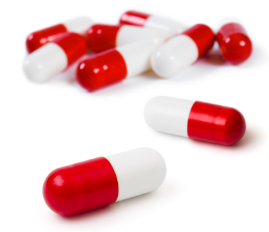
\includegraphics[width=2in]{pills.png}
\end{center}

\noindent The recovery rate right now for patients with the disease is 63\%. Assume this is the truth known with certainty.

\benum
\subquestionwithpoints{2} Bob who has the disease wants to be part of the drug trial. Model Bob's recovery as of now as 1 if he recovers and 0 if he does not recover as a r.v. below. Be sure to indicate parameter value(s). \spc{1} 

\subquestionwithpoints{3} 100 people just like Bob with the disease want to be part of the trial. Model the total number of people of those 100 who will recover as of now below as the r.v. $X$. Be sure to indicate parameter value(s). \spc{1} 

\subquestionwithpoints{4} What two assumptions did you make about the 100 people in order to build the model in part (b)? Explain each in this context. 

\begin{table}[h]
\centering
\begin{tabular}{l|l}
Assumption Name: \hspace{2.0in} & Assumption Name: \hspace{2.0in} \\ \hline
Discussion: & Discussion: \\ 
& \\
& \\
& \\ 
& \\
& \\
& \\
& \\
\end{tabular}
\end{table}

\subquestionwithpoints{2} Calculate the expected number of people of the 100 who will recover.  \spc{1} 

\subquestionwithpoints{3} Compute explicitly the percentage that exactly 63 people will recover. Round to two decimal places. \spc{3} 

%\subquestionwithpoints{3} Why is your answer to (f) so low? Discuss. \spc{3} 

\subquestionwithpoints{5} For those 100 people just like Bob with the disease, model the \textit{proportion} of people who will recover below as the r.v. $\Phat$ and provide its \textit{approximate} distribution. Be sure to indicate parameter values.\spc{5}

\subquestionwithpoints{2} What theorem did you use to answer (h)? No need to discuss. \spc{1} 

\subquestionwithpoints{2} Find $\prob{\Phat = 0.63}$ below assuming the approximate distribution (and not the distribution of the r.v. in part b). \spc{0.1} 

\subquestionwithpoints{2} We will now start testing our drug. Denote the proportion of people who truly recover as the population parameter $p$. We are unsure if the drug works and want to be scientifically honest. Thus our null hypothesis will be that the proportion of people who recover when taking the drug will be \textit{at most} the same as the population overall. Write this in our notation we used in class below. \spc{1}


\subquestionwithpoints{2} Write the alternative hypothesis using the notation we learned in class. \spc{0.1}

\subquestionwithpoints{1} What is the official name of this statistical test? \spc{1}


\subquestionwithpoints{2} We will set $\alpha = 2.5\%$ since the scientific community is very conservative when it comes to new drugs. What is the probability of a Type I error?\spc{2}

\subquestionwithpoints{3} Explain what a Type I error would be in this context.\spc{1}

\subquestionwithpoints{3} Explain what a Type II error would be in this context.\spc{1}

\subquestionwithpoints{3} Discuss what you believe the cost of a type II error would be in this case. \spc{2}

\subquestionwithpoints{5} For the case where we have $n=100$ people who take the drug, find the retainment region for $H_0$ in this hypothesis test. Round to three digits. \spc{8}

\subquestionwithpoints{5} Imagine 72 people of the 100 in the drug trial recovered. Run the hypothesis test, state the conclusion and then write a sentence which explains your conclusion in the context of drug trial. \spc{4}


\subquestionwithpoints{1} Regardless of the conclusion of the hypothesis test, you \emph{feel} deep down inside that the drug is effective in increasing the recovery rate of the disease. What type of error do you \emph{feel} you made here? No explanation necessary. \spc{1}


\subquestionwithpoints{3} If you were to design another experiment to prove that the drug is effective, what would you do differently and why? Hint: increasing $\alpha$ is \textit{not} the answer. \spc{3}

\subquestionwithpoints{2} Regardless of the conclusion of the hypothesis test, we will pretend that the point estimate you computed, i.e. $\phat = 0.72$, represents the real probability of recovery under the drug. Denote $R$ as the event of recovery and $D$ as the event that the drug was taken. Thus $R^C$ denotes the person did not recover and $D^C$ denotes the person did not take the drug. What is $\cprob{R}{D}$? \spc{1}

\subquestionwithpoints{1} Find $\cprob{R^C}{D}$.\spc{2}

\subquestionwithpoints{6} Let's say the drug is on the market and you estimate 20\% of the people who have the disease take the drug. You see someone who recovers, what is the probability they took the drug? \spc{7}

\eenum


\problem You are part of a call center for a very large company.

\begin{center}

\includegraphics[width=4in]{call.png}
\end{center}

\noindent You have millions of clients but the probability each of them call in at any moment is very small. If there are 3,000,0000 clients and the probability any of them call in any second is 1 in 1,000,000 then you can say $\lambda = 3$ and model time in seconds until the next call as an \emph{exponential} distribution.

\benum
\subquestionwithpoints{2} Based on the description above, denote the time until the next call as r.v. $X$. Notate its distribution below as $X \sim$ something.\spc{5}

\subquestionwithpoints{4} Provide a rough illustration of $f(x)$. Label the axes and label one point on the y-axis that is not 0. Do not worry about scale. \spc{6}

\subquestionwithpoints{4} Provide a rough illustration of $F(x)$. Label the axes and label one point on the y-axis that is not 0. Do not worry about scale.  \spc{5}


\subquestionwithpoints{4} What is the probability we will wait more than 5 seconds for the next call that comes in? No need to compute explicitly. \spc{3}

\subquestionwithpoints{4} 4 seconds just elapsed. Given this information, what is the probability we will wait more than 5 seconds for the next call that comes in? No need to compute explicitly. \spc{3}

\eenum



\problem Some theoretical exercises are below.


\benum
\subquestionwithpoints{3} On the homework you were introduced to the r.v. $X \sim \poisson{\lambda}$. The PMF is $p(x) = \lambda^x e^{-\lambda} / x!$. If $\support{X} = \naturals \cup \braces{0}$, write an expression for $\expe{X}$ but \textit{do not solve}.\spc{2}

\subquestionwithpoints{5} On the homework you were given that if $X \sim \poisson{\lambda}$ then $M_X(t) = e^{\lambda(e^t - 1)}$. Find $\expe{X}$ by any way you believe to be best.\spc{5}


\subquestionwithpoints{3} Calculate 

\beqn
\int_2^\infty \oneoversqrt{2\pi} e^{-\half\squared{x-2}}dx = \quad\quad\quad\quad\quad\quad\quad\quad\quad\quad\quad\quad\quad\quad\quad\quad\quad\quad\quad\quad\quad\quad\quad\quad\quad\quad\quad\quad
\eeqn\spc{3}

\subquestionwithpoints{2} Let $X \sim \uniform{0}{1}$. Compute $\se{X}$ to two decimal places.\spc{3}


\subquestionwithpoints{2} Assume $\prob{A} > 0$. Compute $\cprob{A}{A}$. \spc{2}

\subquestionwithpoints{5} You are riding the F train from Roosevelt Ave Jackson Heights to Forest Hills 71Av/Continental. 


\begin{center}
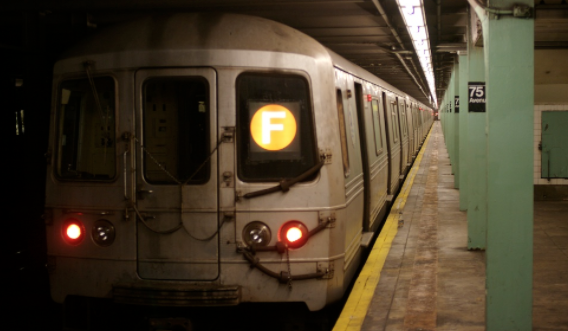
\includegraphics[width=5in]{f_train.png}
\end{center}

\noindent That means you are traveling for 6 stops. The traveling time of each stop can be modeled as a r.v. with distribution $\normnot{1}{0.2042^2}$ minutes and we will assume independent travel time for each stop. Find the probability it takes you more than 7 minutes to get from Roosevelt Ave Jackson Heights to Forest Hills 71Av/Continental.\spc{10}


\subquestionwithpoints{5} [Extra credit] Prove or disprove: $X \sim \uniform{a}{b}$ has the memorylessness property. \spc{7}

\subquestionwithpoints{5} [Extra credit] If $X \sim \poisson{\lambda}$, find $\var{X}$. \spc{7}

\subquestionwithpoints{5} [Extra credit] Find the skewness of the standard normal. 


\eenum

\end{document}

















\problem Imagine a bag with 171 marbles each unique. 

\begin{center}
\includegraphics[width=2in]{marbles.jpg}
\end{center}
\benum

\subquestionwithpoints{3} Imagine you select 19 balls with replacement. How many ways are there to select balls if their order matters and selection order matters? \spc{1} 

\subquestionwithpoints{3} Imagine you select 19 balls with replacement. How many ways are there to select balls if their order does not matter? \spc{1} 

\subquestionwithpoints{3} Imagine you select 19 balls without replacement. How many ways are there to select balls if their order matters? \spc{1} 

\subquestionwithpoints{3} Imagine you select 19 balls without replacement. How many ways are there to select balls if their order does not matter? \spc{1}

%\subquestionwithpoints{2} Although they're all different, 13 of them are red and the red ones are special. If you pull out 10 marbles, how many red ones are you able to get? \spc{1}

%\subquestionwithpoints{3} Although they're all different, 29 of them are red and the red ones are special. If you pull out 150 marbles without replacement, how many red ones are you able to get? \spc{1}

%\subquestionwithpoints{2} What is the probability of getting 11 red ones on a draw of 150 without replacement? No need to compute explicitly. \spc{1}

%\subquestionwithpoints{3} 23 of them are red and the red ones are special. Imagine you have already drawn 10 red marbles on a draw of 10 without replacement. What is the chance you now get another 10 marbles in a draw of 140 without replacement? No need to compute explicitly. \spc{3}

%\subquestionwithpoints{2} Imagine you have already drawn 10 red marbles on a draw of 10 without replacement. What is the chance you now get another 10 marbles in a remaining draw of 140 \textit{with} replacement? No need to compute explicitly. \spc{1}



\eenum

\problem Some theoretical exercises are below.

\benum

\subquestionwithpoints{2} Consider the following r.v.,

\beqn
X \sim \begin{cases}
2 \withprob 1/7 \\
4 \withprob 4/7 \\
-3 \withprob 2/7 \\
\end{cases}
\eeqn

Provide a set $\Omega$ for the domain of this r.v. \spc{1}

\subquestionwithpoints{3} For the r.v. above, describe or illustrate (any way you can) of a physical device that will create the r.v. Be sure to use $\Omega$ in your illustration from (a).\spc{5}

\subquestionwithpoints{2} Could it be possible that $\abss{\support{X}} < \abss{\Omega}$? Write \qu{yes} or \qu{no} only. \spc{1}

\eenum

\problem Some more theoretical exercises are below.

\benum

\subquestionwithpoints{4} Consider $X \sim \uniformdiscrete{a_1, a_2, a_3, a_4}$ i.e. $\abss{\support{X}} = 4$. Find the MGF of $X$ denoted by $M_X(t)$. \spc{2}


\subquestionwithpoints{7} Consider a large number of $X_1, \ldots, X_n \iid \uniformdiscrete{a_1, a_2, a_3, a_4}$. Consider $X_1 + \ldots + X_n$. What is its approximate distribution? Answer in as much detail as you can provide (partial credit will be given). Use sum notation for compactness.  \spc{6}

\subquestionwithpoints{7} Consider $Y_1$ being distributed as 5 or 10 with equal probability and $Y_2 \sim \bernoulli{\half}$ where $Y_1$ and $Y_2$ are independent. Show that $Y_1 + Y_2$ is a uniform discrete r.v. with $\abss{\support{X}} = 4$ using MGF's. \spc{8}



\subquestionwithpoints{3} [E.C.] Give examples of $a_1, a_2, a_3, a_4$ above which would most likely break the approximation from part (d) for a modest size $n$. \spc{2}

\subquestionwithpoints{3} [E.C.] Find $\expe{\tothepow{\frac{X-\mu}{\sigma}}{13}}$ where $\mu$ and $\sigma$ are the mean and standard error of $X$ respectively. \spc{1}

\eenum




\problem We will investigate more about aliens and UFOs by looking at data from the \href{http://www.nuforc.org/webreports/ndxevent.html}{National UFO Reportion Center Online Database}.

\begin{figure}[htp]
\centering
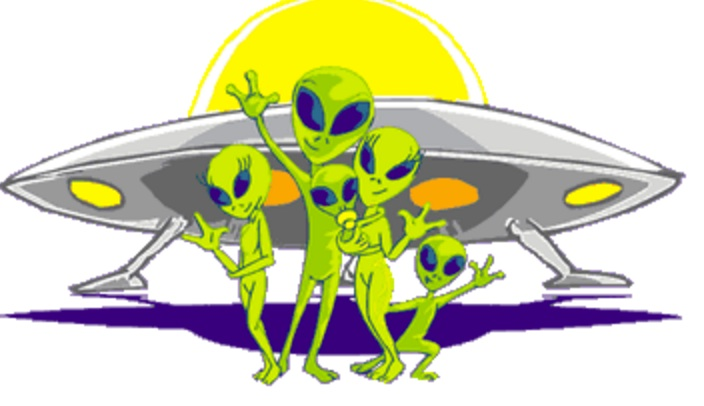
\includegraphics[width=2in]{ufo.jpg}
\end{figure}

Below is the number of events in each month in 2014 and represents the number of \qu{UFO sightings} across America, a country with 319 million people. Assume that each sighting is unique --- that is each person either makes a sighting for a given or does not and there are no duplicates. That is, a person cannot make more than one sighting per 12-month period.

\begin{table}[htp]
\small
\centering
\begin{tabular}{c|c}
Month & Number \\ \hline
12/2014 &	521 \\
11/2014	&543 \\
10/2014	&786 \\
09/2014	&829 \\
08/2014	&922 \\
07/2014	&1096 \\
06/2014	&776 \\
05/2014	&652 \\
04/2014	&666 \\
03/2014	&517 \\
02/2014	&554 \\
01/2014	&715 \\
\end{tabular}
\end{table}

\benum

\subquestionwithpoints{2} We are interested in the true proportion of people who sight a UFO per year (not per month). Provide an estimate of this proportion below. Round to the nearest two digits. \spc{0.5}

\subquestionwithpoints{6} Provide a 99.7\% confidence interval for the true proportion of people worldwide who see a UFO yearly. \spc{5}

\subquestionwithpoints{3} Give two possible concerns as to why the confidence interval you produced in (b) may not be valid.

\begin{enumerate}
\item [1.] ~\\~\\
\item [2.]
\end{enumerate}

\subquestionwithpoints{4} Regardless of the issues in (c), provide four possibe interpretations of the CI from (b).

\begin{enumerate}
\item [1.] ~\\~\\~\\
\item [2.]~\\~\\~\\
\item [3.]~\\~\\~\\
\item [4.]~\\~\\~\\
\end{enumerate}

\subquestionwithpoints{3} Let's assume the point estimate of (a) is equal to the real population proportion (assume $p = \phat$ for the remainder of the problem). Assume 2015 is the same as 2014 with regards to UFO sightings (and the population of America remained the same to the nearest million people). What is the probability of less than 100,000 sightings in 2015? No need to compute exactly. Sum notation allowed.\spc{2}

\subquestionwithpoints{2} It is possible some states have more UFO sightings than other states. Hawaii had 67 sightings in 2014 for a population of 1.42 million people. Here are some examples:

\begin{table}[htp]
\centering
\footnotesize
\begin{tabular}{lllll}
Timestamp & City & Shape & Duration & Description \\ \hline
1/15/14 03:30&	Paia	HI&	Sphere	&2 min	&  I Saw a golden sphere \\
&&&&shaped object hovering over the water \\
&&&&on the North Shore at 3:30am.	 \\
1/15/14&	Kealia	HI	&Fireball	&20 min&	Fireball w- chinese laturns and parade \\
&&&& of triangles.	 \\
1/14/14 20:50&	Waimanalo	HI	&Fireball&	5 sec&	I saw an orange fireball with flames \\
&&&& trailing as it shot diagonally across \\
&&&& the sky and disappeared behind the\\
&&&& nearby mountain range.	 \\ 
%1/10/14 22:58&	Kaneohe	HI&	Fireball&	90 sec&	A silent red ball of light traveled \\
%&&&&off the pacific ocean from the east \\
%&&&&to the south below the clouds for \\
%&&&&about 90 seconds.	 \\
\end{tabular}
\end{table}

Find the sample proportion for seeing a UFO sighting in a year in Hawaii. Round to two digits. \spc{2}

\subquestionwithpoints{7} Test whether this proportion is different than the proportion in America overall.

\begin{enumerate}
\item [$H_0$:] ~\\
\item [$H_a$:] ~\\
\item [$\alpha =$] ~~~~~~~~ $\Rightarrow z_{\alpha/2} = $
\end{enumerate}~ \spc{2.5}

\subquestionwithpoints{2} Based on your result in (g), is the event of being in Hawaii and the event of seeing a UFO over the course of a year independent or dependent? Explain using the definition of dependence and independence. \spc{2}

\eenum


\problem We return to our discussion of Chevalier de Mere and his compulsive dice gambiling.


\begin{figure}[htp]
\centering
\includegraphics[width=1.31in]{chevalier.jpg}~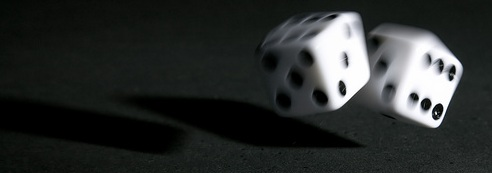
\includegraphics[width=2in]{dice.jpg}
\end{figure}

\benum

\subquestionwithpoints{3} Recall the dice game he played: you win if you get at least one 6-6 in 24 rolls of two dice. What is the probability of winning? Compute to four decimal places. \spc{3}

\subquestionwithpoints{6} Chevalier de Mere most likely thought the probability of winning was 0.5 (not your answer from the previous question). Assuming Chevalier de Mere went easy on the wine and cigarettes and kept perfect records of wins and losses of everyone playing this game, how many games (denoted $n$) did he have to watch to be sure (at the 5\% level) that the probability of winning was less than 50\%. You can leave as an algebraic equation of $n$; you do not need to solve.\spc{7}


\eenum


\problem We learn about a bank alert system here for detecting fraudulent charges on a credit card.
\begin{figure}[htp]
\centering
\includegraphics[width=3in]{credit.jpg}
\end{figure}

\benum

\subquestionwithpoints{2} Assume each charge is legitimate from the start. What are the null and alternative hypotheses for this situation with credit card charges? No credit given for the general definition. Answer in English. \spc{1.5}

%\subquestionwithpoints{2} Describe a Type I error for this situation with credit card charges. No credit given for the general definition. \spc{2}

\subquestionwithpoints{3} Describe a Type II error for this situation with credit card charges. No credit given for the general definition. Answer in English. \spc{2}

\subquestionwithpoints{3} Assume the Type I error rate is $\alpha$ with cost $C_I \sim \normnot{\$100}{\$50^2}$ and the Type II error rate is $\beta$ with cost $C_{II} \sim \normnot{\$500}{\$38^2}$. What is the expected cost to the bank for a single credit card transaction? \spc{3}

%\subquestionwithpoints{3} Assuming the bank cannot change the two costs ($C_I$ and $C_{II}$). Give a strategy for the bank to minimize the expected cost in (d) without any chance of inadvertently increasing it. \spc{1}


\eenum



\problem Some questions about continuous r.v.'s

\benum


\subquestionwithpoints{2} The chi-squared distribution (denoted $\chi^2_k$) has a PDF given by

\beqn
\chi^2_k := f(x) = \frac{1}{2^{\frac{k}{2}}\Gamma\left(\frac{k}{2}\right)}\; x^{\frac{k}{2}-1} e^{-\frac{x}{2}}
\eeqn 

and its support is all non-negative numbers. Note that the gamma function (denoted $\Gamma$) is evaluated to a number using a computer.  \\

What are the parameter(s) of the $\chi^2_k$ model?\spc{2}

\subquestionwithpoints{4} Write an integral expression for $\expe{X}$ where $X \sim  \chi^2_k$. \spc{4}

\subquestionwithpoints{4} Write an integral expression for $F(x)$ where $X \sim  \chi^2_k$. \spc{4}

\subquestionwithpoints{3} Consider $T \sim \exponential{\lambda}$ which represents the time spent waiting for the Q64 in minutes. What is the probability of waiting more than 10 minutes? \spc{3}

\subquestionwithpoints{4} A stopwatch beeps every minute. After each beep, which r.v. models the waiting time in minutes for the Q64? Assume of course the bus hasn't come by the beep.  \spc{2}

%\subquestionwithpoints{2} A stopwatch beeps every 1$\mu$s (that's one-millionth of a second). After each beep, which r.v. models the waiting time in minutes for the Q64? Assume of course the bus hasn't come by the beep.  \spc{2}

\eenum

\problem Some theoretical questions below


\end{document}

